\section{Outline}
\subsection{Requirements} 
\paragraph{Physics requirements} 
\paragraph{Technical specs} 
\subsection{Design}
\paragraph{Barrel layout, support structure}
\paragraph{Module design}
\paragraph{Deflection}
\paragraph{Thermal analysis and heat removal}
\paragraph{Module Assembly and QA}
\subsection{Hardware}
\paragraph{Cooling system}
\paragraph{Purging system}
\paragraph{Slow controls, interlocks, and monitoring, detector safety}
\subsection{Electronics}
\paragraph{Grounding and shielding}
\paragraph{Power supplies}
\paragraph{Crates (VXS, VME, MPOD)}
\subsection{Readout}
\paragraph{Front-end electronics, FSSR2}
\paragraph{VSCM}
\paragraph{DAQ}
\subsection{Calibration}
\paragraph{Calibration algorithm}
\paragraph{Calibration plots}
\subsection{Reconstruction}
\paragraph{Local reconstruction, clustering}
%\paragraph{Track reconstruction}
\subsection{Simulation}
%\paragraph{Expected physics performance}
\paragraph{Backgrounds, Energy deposition, Dose rates}
\paragraph{Occupancies}
%\paragraph{Alignment}
%\paragraph{Resolutions}
%\paragraph{Efficiencies}
\subsection{Performance}
\paragraph{Module testing (QA, full chain, r/a sources, beam)}
\paragraph{Integration and system checkout}
\paragraph{Cosmic rays}
\paragraph{Commissioning with beam}
%\paragraph{Tracking performance, resolution, efficiency}
\subsection{Conclusion}
\subsection{References}

\newpage
\section{Overview}

Deep exclusive reactions, in which an electron scattering results in a meson-baryon final state, provide stringent requirements for the CLAS12 tracking system. The central tracker consists of a solenoid, Central Time-Of-Flight system (CTOF), and Central Vertex Tracker (CVT). The CVT is centered inside of the  5~T solenoid magnet and consists of the inner Silicon Vertex Tracker (SVT) and the Barrel Micromegas Tracker (BMT). CVT reconstructs low energy hadrons at large polar angles and has tight constrains on material budget to minimize energy loss due to multiple scattering.

\begin{wrapfigure}{l}{0.5\columnwidth}
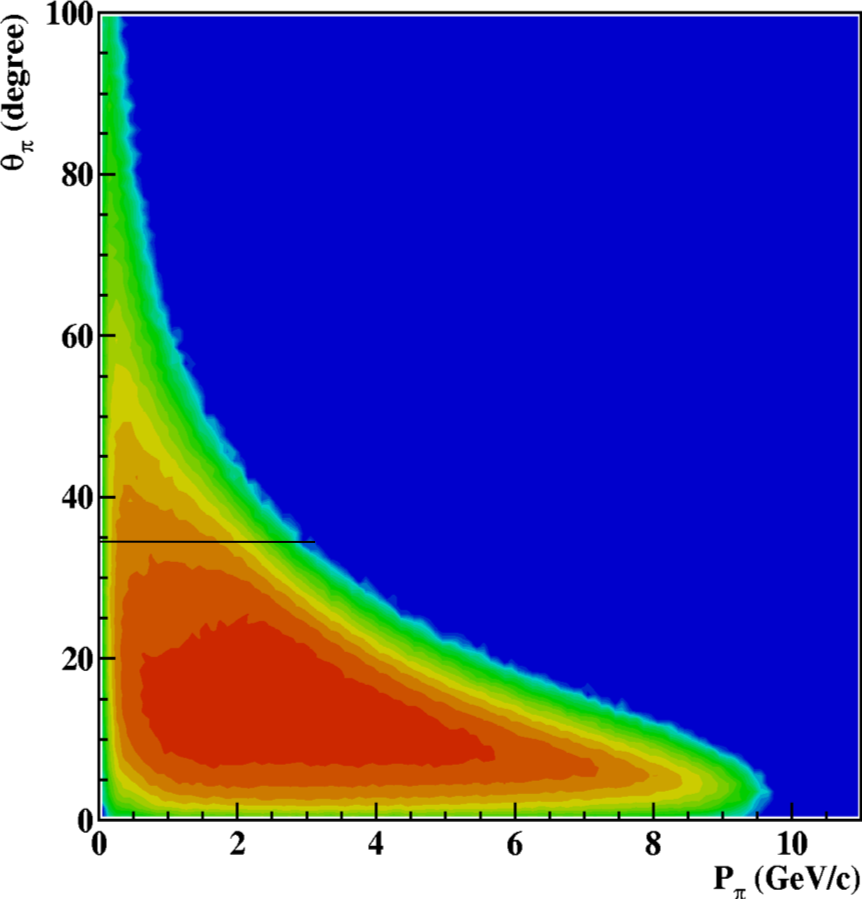
\includegraphics[width=0.5\columnwidth]{clas-momentum.png}
\caption{CLAS12 charged hadron momentum distribution}
\label{fig:clas-momentum}
\end{wrapfigure}

